\subsection{Addressing}

The ECDSA public key acts as a unique identifier for each node in the network. It is structured using \href{https://github.com/multiformats/multiformats}{multiformats} by Protocol Labs and encoded using \href{https://en.bitcoin.it/wiki/Base58Check_encoding}{Base58} encoding, known from Bitcoin. The structure is given by the multiformats prefix \textsf{0x002508021221} and the compressed ECDSA public key, leading to an identifier $id$ of 39 bytes and

\begin{center}
    $id = base58.encode(\mathsf{0x002508021221} \ || \ \mathsf{pubKey})$
\end{center}

Identifiers distinguish nodes from each other, whereas addresses allow nodes to establish a connection to each other. HOPR distinguishes two types of addresses: direct addresses and relay addresses. Both address types are structured using \href{https://github.com/multiformats/multiaddr}{multiaddr} by Protocol Labs.

\paragraph{Direct Addresses}

Each nodes that is able to listen directly to a TCP socket determines its own direct addresses. These include its local IP address, e.g. \textsf{127.0.0.1}, its local IP address, e.g. \textsf{192.168.0.2} as well as, if available, its public IP address, e.g. \textsf{1.2.3.4}. A node with identifier $id$ and public IP address \textsf{1.2.3.4} listening to TCP port $9091$ has the addr

\begin{center}
    \textsf{/ip4/1.2.3.4/tcp/9091/}\textless$id$\textgreater{}
\end{center}

\paragraph{Relay Addresses}

As many consumer routers hide connected nodes due to security concerns, and the scarcity of IPv4 addresses, behind a NAT, these nodes cannot reach each other directly because they do not know how to bypass the other party's NAT mechanism.

\begin{figure}[H]
    \centering
    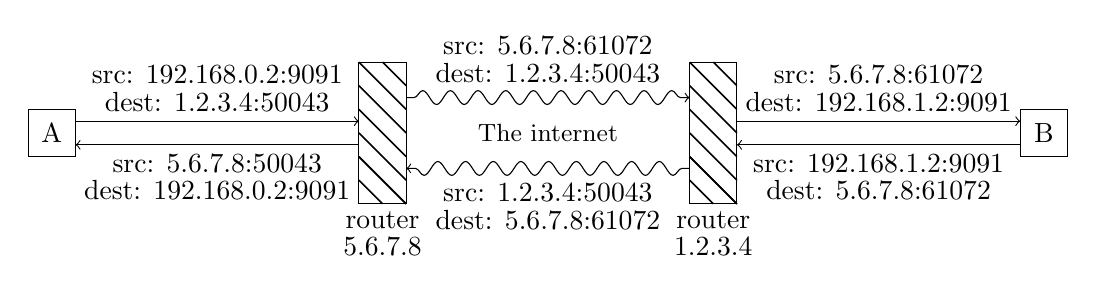
\begin{tikzpicture}
        \def\nodeWidth{0.6}
        \def\nodeHeight{0.6}
        \def\routerWidth{0.6}
        \def\routerHeight{1.8}
        \def\routerOffset{4.2}

        % Subnet A
        \draw (0,0) rectangle (\nodeWidth,\nodeHeight) node[midway] {A};

        % Interaction with router A
        \draw[->] (\nodeWidth,0.75*\nodeHeight) -- (\routerOffset,0.75*\nodeHeight) node[midway,above] {\smaller{\shortstack{src: 192.168.0.2:9091\\dest: 1.2.3.4:50043}}};

        \draw[->] (\routerOffset,0.25*\nodeHeight) -- (\nodeWidth,0.25*\nodeHeight) node[midway,below] {\smaller{\shortstack{src: 5.6.7.8:50043\\dest: 192.168.0.2:9091}}};

        % Router to router interaction
        \begin{scope}[shift={(0,-0.6)}]
            \draw[->,decorate,decoration={snake,pre length=1mm,post length=1mm}] (\routerOffset+\routerWidth,0.75*\routerHeight) -- (2*\routerOffset,0.75*\routerHeight) node[midway,above=2pt] {\smaller{\shortstack{src: 5.6.7.8:61072\\dest: 1.2.3.4:50043}}};
            \draw[->,decorate,decoration={snake,pre length=1mm,post length=1mm}] (2*\routerOffset,0.25*\routerHeight) -- (\routerOffset+\routerWidth,0.25*\routerHeight) node[midway,below=2pt] {\smaller{\shortstack{src: 1.2.3.4:50043\\dest: 5.6.7.8:61072}}};

            \path (\routerOffset+\routerWidth,0.5*\routerHeight) -- (2*\routerOffset,0.5*\routerHeight) node[midway] {\small{The internet}};
        \end{scope}

        % Subnet B
        \begin{scope}[shift={(3*\routerOffset,0)}]
            \draw (0,0) rectangle (\nodeWidth,\nodeHeight) node[midway] {B};
            % Interaction with router B
            \draw[->] (-\routerOffset+\routerWidth,0.75*\nodeHeight) -- (0,0.75*\nodeHeight) node[midway,above] {\smaller{\shortstack{src: 5.6.7.8:61072\\dest: 192.168.1.2:9091}}};

            \draw[->] (0,0.25*\nodeHeight) -- (-\routerOffset+\routerWidth,0.25*\nodeHeight) node[midway,below] {\smaller{\shortstack{src: 192.168.1.2:9091\\dest: 5.6.7.8:61072}}};
        \end{scope}

        \foreach \offset\name\address in{1/A/5.6.7.8,2/B/1.2.3.4} {
                \begin{scope}[shift={(\offset*\routerOffset,-0.6)}]
                    \def\a{0.6}
                    \def\b{1.8}
                    \def\diff{1.2}

                    \def\lw{0.2}

                    \foreach \x [count=\i] in{0,0.3,0.6,...,\a}{
                            \draw [line width=\lw mm](\x,0)--(0,\x) (\x,\b)--(\a,\b-\a+\x);
                        }
                    \foreach \x [count=\i] in{0,0.3,0.6,...,\diff}{
                            \draw [line width=\lw mm](0,\a+\x)--(\a,\x);
                        }
                    \draw (0,0) rectangle  node[below=25pt] {\smaller{\shortstack{router\\\address}}} (\routerWidth,\routerHeight);
                \end{scope}

            }
    \end{tikzpicture}
    \label{fig:successful-nat-traversal}
    \caption{Successful NAT traversal between A and B after exchanging connection information.}
\end{figure}

To circumvent this problem, HOPR nodes can also dial each other using \textit{relay addresses}. Each node therefore maintains a list of usable relays which can be used to establish a relayed connection through the relay to the node, yielding addresses like

\begin{center}
    \textsf{/p2p/}\textless\textsf{$relayId$}\textgreater\textsf{/p2p-circuit/p2p/}\textless{}\textsf{$id$}\textgreater{}
\end{center}

where $relayId$ is the identifier of the utilized relay and $id$ is the identifier of the node. Another node who intends to connect to the node with identifier $id$ first connects to the node with identifier $relayId$. This needs to happen by using a direct address. Once the connection has been established, it asks the node with $relayId$ to extend the connection to node with $id$.
